\documentclass{article}
\usepackage{../assignment_preamble}

\title{Homework 3}
\author{Ravi Kini}
\date{November 24, 2025}

\begin{document}

\maketitle

\problem{}
Let $f : \mathbb{R} \to \mathbb{R}$ with $f(x_*) = f'(x_*) = 0$, $f''(x_*) \neq 0$ such that $f'''$ is continuous on an interval around $x_*$. Since the continuity of $f'''$ implies the continuity of $f'$, for any constant $M$, we can select $\delta_1 > 0$ such that for all $x$ such that $|x - x_*| < \delta_1$, $|f(x) - f(x_*)| = |f(x)| < M$. We can also select $\delta_2 > 0$ such that $x_*$ is the only root of $f(x)$ in $[x_* - \delta_2, x_* + \delta_2]$. It then follows that $x_*$ is the only fixed point of:
\begin{align*}
    T(x) = x - \frac{f(x)}{f'(x)}
\end{align*}
in $[x_* - \delta_2, x_* + \delta_2]$. Letting $\delta = \min(\delta_1, \delta_2)$, by the Fixed-Point Theorem, for any $x_0 \in [x_* - \delta, x_* + \delta]$, the sequence where $x_{k + 1} = T(x_k)$ converges to $x_*$. It then follows that Newton's method converges for $x_0$ sufficiently close to $x_*$, i.e. $x_0 \in [x_* - \delta, x_* + \delta]$.

We now let $f(x) = {(x - x_*)}^2g(x)$, where $g(x_*) \neq 0$ and $g$ is differentiable. Since $x_*$ is the only root in the interval, that $g(x_k) \neq 0$ for $x_k \neq x$. Then:
\begin{align*}
    f'(x) = 2(x - x_*)g(x) + {(x - x_*)}^2g'(x)
\end{align*}
Consequently, letting $e_k = |x_k - x_*|$, we see that:
\begin{align*}
    e_{k + 1} = |x_{k+1} - x_*| & = \left|x_k - \frac{f(x_k)}{f'(x_k)} - x_*\right| \\
    & = \left|x_k - \frac{{(x_k - x_*)}^2g(x_k)}{2(x_k - x_*)g(x_k) + {(x_k - x_*)}^2g'(x_k)} - x_*\right| \\
    & = \left|(x_k - x_*) - \frac{(x_k - x_*)g(x_k)}{2g(x_k) + (x_k - x_*)g'(x_k)}\right| \\
    & = \left|1 - \frac{g(x_k)}{2g(x_k) + (x_k - x_*)g'(x_k)}\right|e_k \\
    & = \left|\frac{g(x_k) + (x_k - x_*)g'(x_k)}{2g(x_k) + (x_k - x_*)g'(x_k)}\right|e_k \\
    \frac{e_{k+1}}{e_k} & = \left|\frac{g(x_k) + (x_k - x_*)g'(x_k)}{2g(x_k) + (x_k - x_*)g'(x_k)}\right|
\end{align*}
Taking the limit as $k \to \infty$, since $\lim_{k\to\infty} x_k - x_* = 0$:
\begin{align*}
    \lim_{k\to\infty} \frac{e_{k+1}}{e_k} & = \lim_{k\to\infty} \left|\frac{g(x_k) + (x_k - x_*)g'(x_k)}{2g(x_k) + (x_k - x_*)g'(x_k)}\right| \\
    & = \lim_{k\to\infty} \frac{1}{2}\left|\frac{2g(x_k) + 2(x_k - x_*)g'(x_k)}{2g(x_k) + (x_k - x_*)g'(x_k)}\right| \\
    & = \lim_{k\to\infty} \frac{1}{2}\left|1 + \frac{(x_k - x_*)g'(x_k)}{2g(x_k) + (x_k - x_*)g'(x_k)}\right| \\
    & = \frac{1}{2}
\end{align*}

\clearpage
\problem{}
\begin{lstlisting}[language=Python]
import numpy as np
import matplotlib.pyplot as plt

def newton(f, J, x0, tol_f=1e-6, tol_dx=1e-6, max_iter=100, line_search=True):
    x = x0.copy()
    history = np.zeros((max_iter, 3))
    for k in range(max_iter):
        fx = f(x)
        Jx = J(x)
        
        norm_f = np.linalg.norm(fx)
        if norm_f < tol_f:
            history[k] = (k, norm_f, 0.0)
            return x, True, k, history
        
        try:
            dx = np.linalg.solve(Jx, -fx)
        except:
            return x, False, k, history
        norm_dx = np.linalg.norm(dx)
        
        alpha = 1
        if line_search:
            alpha = backtracking_line_search(f, x, fx, dx, norm_f)
        
        x_new = x + alpha * dx
        history[k] = (k, norm_f, norm_dx)
        if norm_dx < tol_dx:
            return x_new, True, k + 1, history
        x = x_new.copy()
    return x, False, max_iter, history

def backtracking_line_search(f, x, fx, dx, norm_f, rho=0.5, c=1e-4, max_iter=20):
    alpha = 1
    norm_f_sq = norm_f ** 2
    phi_prime_0 = -norm_f_sq
    for _ in range(max_iter):
        x_new = x + alpha * dx
        fx_new = f(x_new)
        norm_f_new_sq = np.linalg.norm(fx_new) ** 2
        
        if norm_f_new_sq <= norm_f_sq + c * alpha * phi_prime_0:
            return alpha
        
        alpha *= rho
    return alpha
\end{lstlisting}

\subproblem{(a)}
\begin{align*}
    f(x_1, x_2) = \left(\frac{5 - 2x_1}{2x_2 - 3}, \frac{5 - 2x_2}{2x_1 - 3}\right)
\end{align*}
For $x_0 = (1, 1)$:
\begin{center}
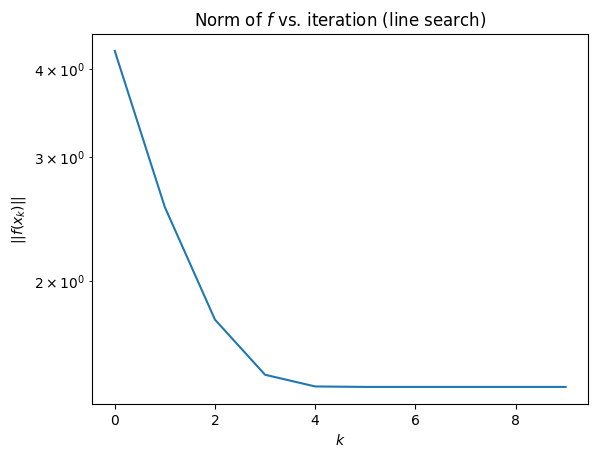
\includegraphics[width=0.45\textwidth]{../../img/mat226a/hw_3_2a-1.png}
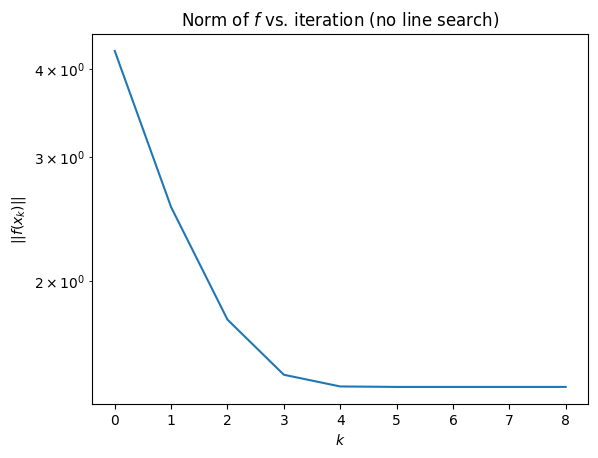
\includegraphics[width=0.45\textwidth]{../../img/mat226a/hw_3_2a-2.png}
\end{center}
For $x_0 = (3, 3)$:
\begin{center}
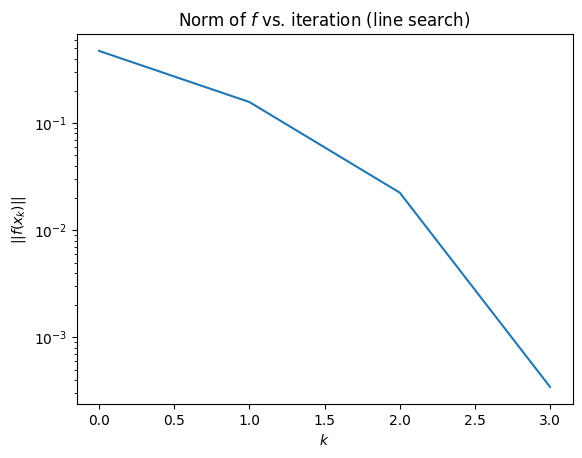
\includegraphics[width=0.45\textwidth]{../../img/mat226a/hw_3_2a-3.png}
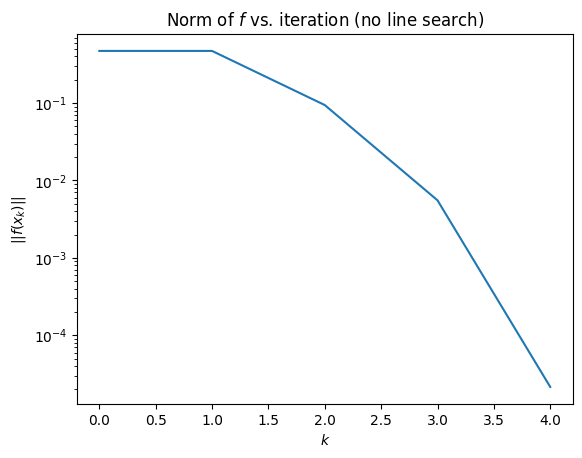
\includegraphics[width=0.45\textwidth]{../../img/mat226a/hw_3_2a-4.png}
\end{center}
For $x_0 = (10, 10)$:
\begin{center}
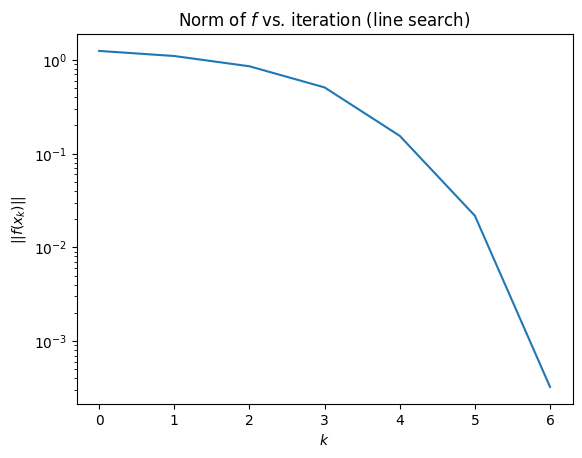
\includegraphics[width=0.45\textwidth]{../../img/mat226a/hw_3_2a-5.png}
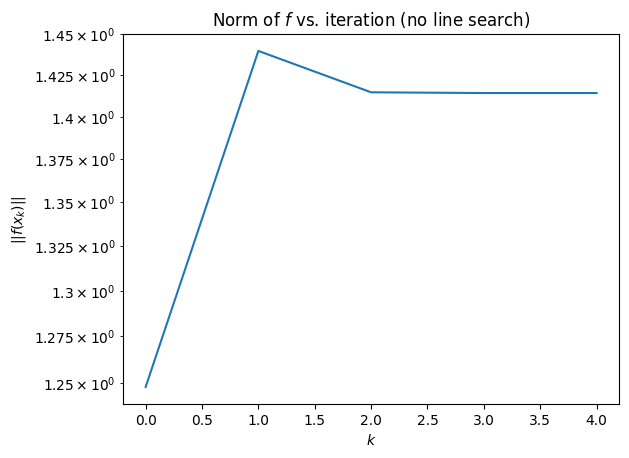
\includegraphics[width=0.45\textwidth]{../../img/mat226a/hw_3_2a-6.png}
\end{center}

The system has singularities when $x_1 = 3/2$ or $x_2 = 3/2$, and the root is at $(x_1, x_2) = (5/2, 5/2)$. For an initial guess of $x_0 = (1, 1)$, which is closer to the singularity, Newton's method converges to a point close to $(0, 0)$ both with and without line search. For an initial guess of $x_0 = (3, 3)$, which is equally close to both the root and the singularity, Newton's method converges to the root, although it does so faster using line search. For an initial guess of $x_0 = (10, 10)$, which is far from both the root and the singularity, Newton's method converges to the root with line search and to a point close to $(0, 0)$ without line search. Line search is useful when a singularity is present, helping Newton's method to navigate away from the singularity.

\subproblem{(b)}
\begin{align*}
    f(x) = \frac{x^2}{1 + x^2}
\end{align*}
For $x_0 = 1$:
\begin{center}
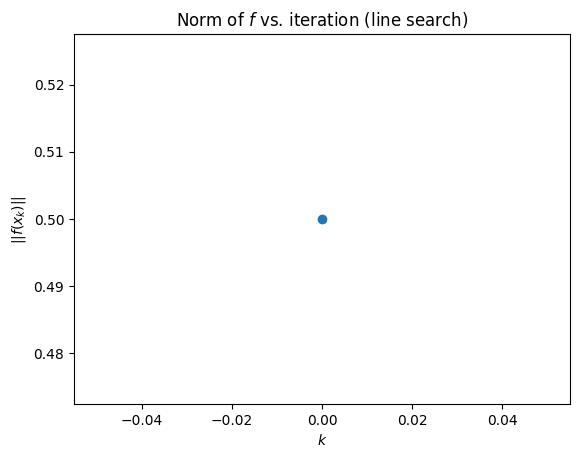
\includegraphics[width=0.45\textwidth]{../../img/mat226a/hw_3_2b-1.png}
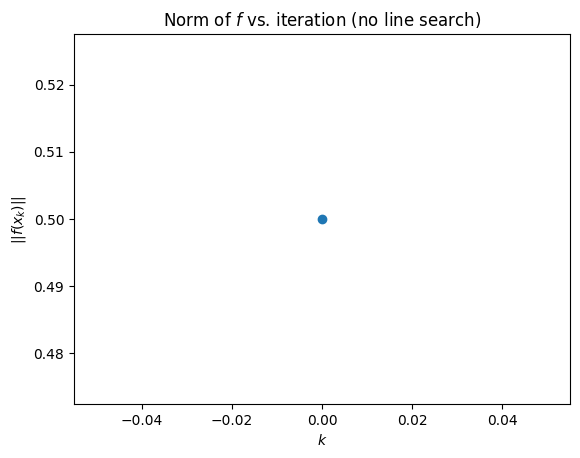
\includegraphics[width=0.45\textwidth]{../../img/mat226a/hw_3_2b-2.png}
\end{center}
For $x_0 = 10$:
\begin{center}
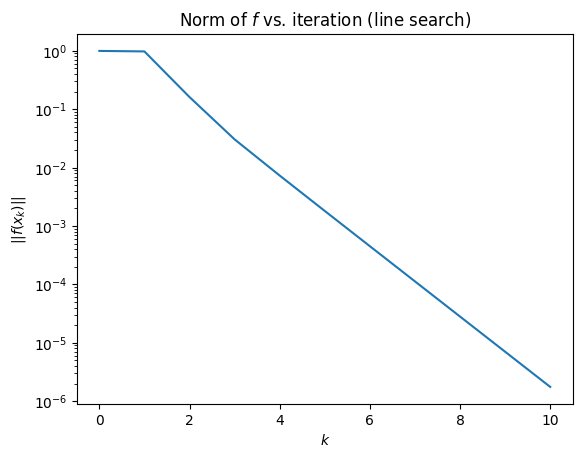
\includegraphics[width=0.45\textwidth]{../../img/mat226a/hw_3_2b-3.png}
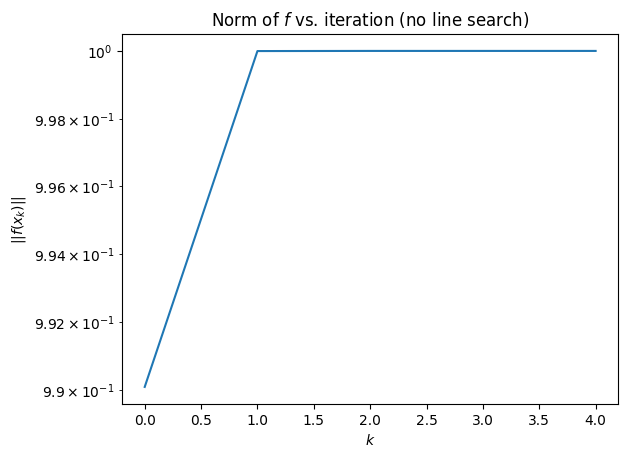
\includegraphics[width=0.45\textwidth]{../../img/mat226a/hw_3_2b-4.png}
\end{center}

The system has no singularities, and the root is at $x = 0$. For large $x$, $f'(x) \approx 0$. For an initial guess of $x_0 = 1$, which is close to the root, Newton's method converges after one iteration, both with and without line search. For an initial guess of $x_0 = 10$, which is far from the root, Newton's method converges to the root with line search, and diverges without line search. Line search is useful when the function has a small gradient, resulting in very large steps.

\subproblem{(c)}
\begin{align*}
    f(x_1, x_2) = \left(x_1x_2 + x_1^3 + 4, x_1x_2^2 + x_2 + 6\right)
\end{align*}
For $x_0 = (-1, -1)$:
\begin{center}
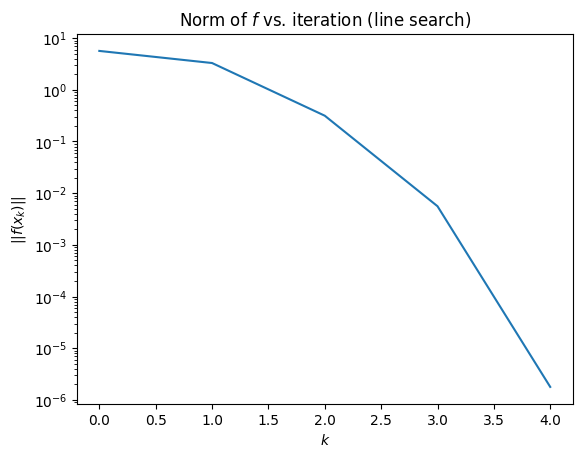
\includegraphics[width=0.45\textwidth]{../../img/mat226a/hw_3_2c-1.png}
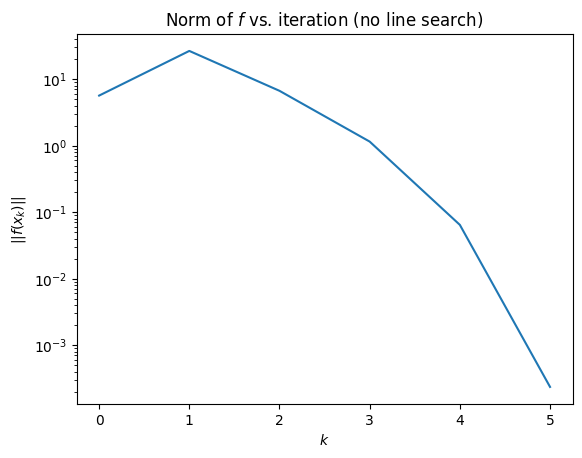
\includegraphics[width=0.45\textwidth]{../../img/mat226a/hw_3_2c-2.png}
\end{center}
For $x_0 = (1, 1)$:
\begin{center}
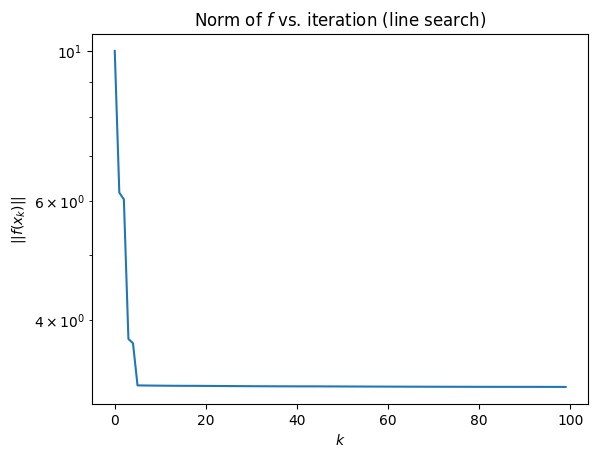
\includegraphics[width=0.45\textwidth]{../../img/mat226a/hw_3_2c-3.png}
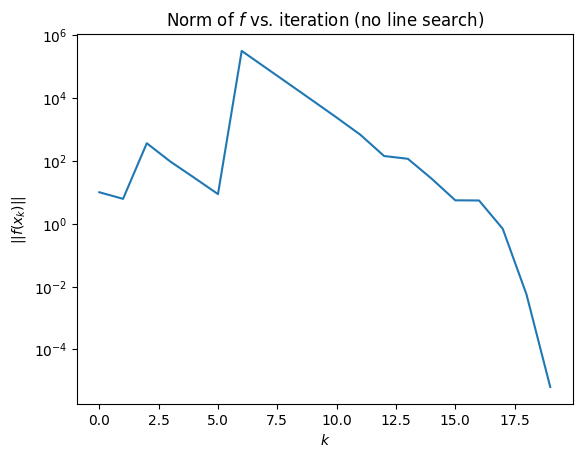
\includegraphics[width=0.45\textwidth]{../../img/mat226a/hw_3_2c-4.png}
\end{center}

The system has no singularities, and the roots are at $(x_1, x_2) = (-1, 3)$ and $(x_1, x_2) \approx (-1.905, -1.531)$. For an initial guess of $x_0 = (-1, -1)$, which is close to both, Newton's method converges to a point close to the second root both with and without line search. For an initial guess of $x_0 = (1, 1)$, which is farther, Newton's method does not converge with line search, and converges to the first root without line search.

\clearpage
\problem{}
\subproblem{(a)}
\begin{lstlisting}[language=Python]
eps = 1e-3
g = 0.25

N = 100
dx = 1 / (N + 1)
x = np.linspace(dx, 1 - dx, N)

coeff = eps / (dx ** 2)
A = np.zeros((N, N))

for i in range(N):
    A[i, i] = -2 * coeff
    if i > 0:
        A[i, i-1] = coeff
    if i < N - 1:
        A[i, i+1] = coeff

def F(u):
  return -np.exp(-np.abs(u)) * u + g

def dFdu(u):
  result = np.zeros_like(u)
  mask_pos = u > 0
  mask_neg = u < 0
  mask_zero = np.abs(u) < 1e-10
  
  result[mask_pos] = -np.exp(-np.abs(u[mask_pos])) * (1 - u[mask_pos])
  result[mask_neg] = -np.exp(-np.abs(u[mask_neg])) * (1 + u[mask_neg])
  result[mask_zero] = -1.0
  return result

def J(u):
  return A + np.diag(dFdu(u))

def residual(u):
  return np.dot(A, u) + F(u)

x_final = np.linspace(0, 1, N + 2)

u0 = np.ones(N) * g
u1, converged, iter, history = newton(residual, J, u0, line_search=True)
u1_final = np.zeros(N + 2)
u1_final[1:-1] = u1

u0 = -g * x * (1 - x) / (2 * eps)
u2, converged, iter, history = newton(residual, J, u0, line_search=True)
u2_final = np.zeros(N + 2)
u2_final[1:-1] = u2

plt.plot(x_final, u1_final)
plt.title('Solution 1 (small $u$)')
plt.xlabel('x')
plt.ylabel('u')
plt.show()

plt.plot(x_final, u2_final)
plt.title('Solution 2 (large $u$)')
plt.xlabel('x')
plt.ylabel('u')
plt.show()
\end{lstlisting}
\begin{center}
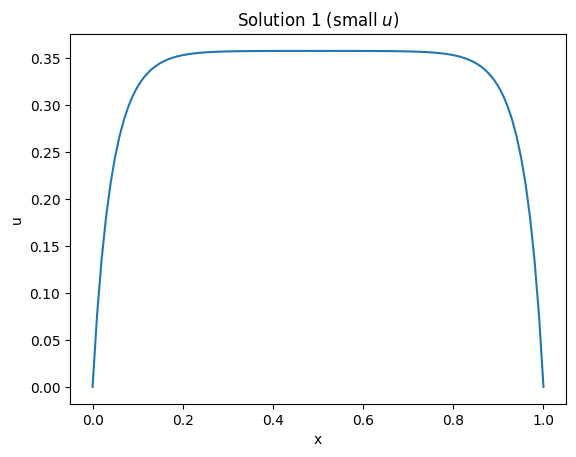
\includegraphics[width=0.45\textwidth]{../../img/mat226a/hw_3_3a-1.png}
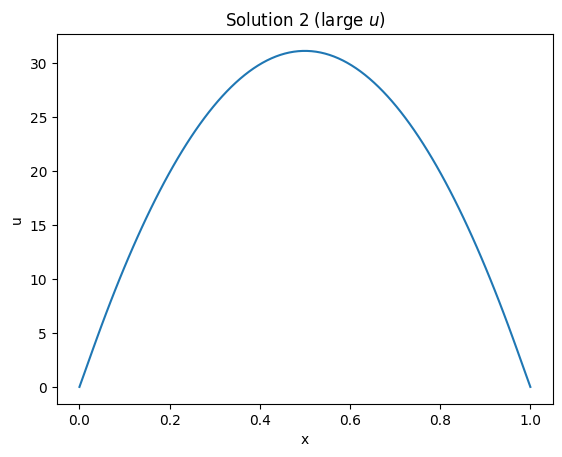
\includegraphics[width=0.45\textwidth]{../../img/mat226a/hw_3_3a-2.png}
\end{center}

\subproblem{(b)}
\begin{lstlisting}[language=Python]
M = 1000
alpha_low = 0.1
alpha_high = 0.9
norms = np.zeros(M)
for a in range(M):
  alpha = alpha_low + (alpha_high - alpha_low) * a / M
  u0 = (1 - alpha) * u1 + alpha * u2
  norms[a] = np.linalg.norm(residual(u0))
alpha = alpha_low + (alpha_high - alpha_low) * np.argmax(norms) / M
u3 = (1 - alpha) * u1 + alpha * u2
u3_final = np.zeros(N + 2)
u3_final[1:-1] = u3

plt.plot(x_final, u3_final)
plt.title('Solution 3 (linear combination)')
plt.xlabel('x')
plt.ylabel('u')
plt.show()
\end{lstlisting}
\begin{center}
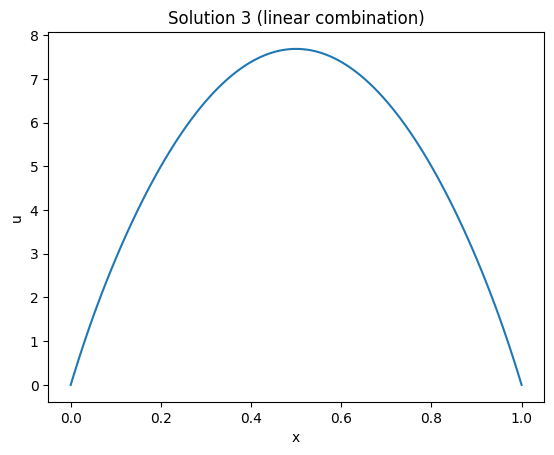
\includegraphics[width=0.75\textwidth]{../../img/mat226a/hw_3_3b.png}
\end{center}

\clearpage
\problem{}
\subproblem{(a)}
\begin{lstlisting}[language=Python]
m = 50
n = 12
x = np.linspace(0, 1, m)
A = np.vander(x, n)
b = np.cos(4 * x)

print(np.linalg.cond(A))
\end{lstlisting}
The condition number of $A$ is approximately $\mathrm{cond}(A) \approx 1.172 \cdot 10^8$.

\subproblem{(b)}
\begin{lstlisting}[language=Python]
def classical_GS(A):
  m, n = A.shape
  Q = np.zeros((m, n))
  R = np.zeros((n, n))

  for j in range(n):
    v = A[:, j].copy()
    for i in range(j):
      R[i, j] = np.dot(Q[:, i], v)
      v -= R[i, j] * Q[:, i]
    R[j, j] = np.linalg.norm(v)
    if R[j, j] > 1e-14:
      Q[:, j] = v / R[j, j]
    else:
      Q[:, j] = v
  return Q, R

def modified_GS(A):
  m, n = A.shape
  Q = A.copy()
  R = np.zeros((n, n))

  for j in range(n):
    R[j, j] = np.linalg.norm(Q[:, j])
    if R[j, j] > 1e-14:
      Q[:, j] /= R[j, j]
    for k in range(j + 1, n):
      R[j, k] = np.dot(Q[:, j], Q[:, k])
      Q[:, k] -= R[j, k] * Q[:, j]
  return Q, R

def householder(A):
  m, n = A.shape
  Q = np.eye(m)
  R = A.copy()

  for j in range(n):
    x = R[j:, j]
    e1 = np.zeros_like(x)
    e1[0] = 1
    v = x + np.sign(x[0]) * np.linalg.norm(x) * e1
    v_norm = np.linalg.norm(v)
    if v_norm > 1e-14:
      v /= v_norm
      R[j:, j:] -= 2 * np.outer(v, np.dot(v, R[j:, j:]))
      Q[:, j:] -= 2 * np.outer(np.dot(Q[:, j:], v), v)
  return Q[:, :n], R[:n, :]
\end{lstlisting}
Since $Q$ should be orthogonal, $Q^T Q - I = 0$. For the classical Gram-Schmidt method, the computed $||Q^T Q - I||_2 \approx 4.881 \cdot 10^{-9}$. For the modified Gram-Schmidt method, the computed $||Q^T Q - I||_2 \approx 4.881 \cdot 10^{-9}$. For the Householder method, the computed $||Q^T Q - I||_2 \approx 1.486 \cdot 10^{-15}$. The matrix computed using the Householder method has the lowest norm since it is backwards stable.

\subproblem{(c)}
\begin{lstlisting}[language=Python]
x = np.linalg.solve(np.matmul(np.transpose(A), A), np.matmul(np.transpose(A), b))
print(np.linalg.norm(x - a))
print(np.linalg.norm(np.matmul(A, x) - b))

Q, R = classical_GS(A)
x = np.linalg.solve(R, np.matmul(np.transpose(Q), b))
print(np.linalg.norm(x - a))
print(np.linalg.norm(np.matmul(A, x) - b))

Q, R = modified_GS(A)
x = np.linalg.solve(R, np.matmul(np.transpose(Q), b))
print(np.linalg.norm(x - a))
print(np.linalg.norm(np.matmul(A, x) - b))

Q, R = householder(A)
x = np.linalg.solve(R, np.matmul(np.transpose(Q), b))
print(np.linalg.norm(x - a))
print(np.linalg.norm(np.matmul(A, x) - b))

x = np.linalg.lstsq(A, b)[0]
print(np.linalg.norm(x - a))
print(np.linalg.norm(np.matmul(A, x) - b))
\end{lstlisting}
\begin{center}
\begin{tabular}{|c|c|c|}
    \hline
    Method & $||x - a||_2$ & $||Ax - b||_2$ \\
    \hline
    Normal equations & $1.654 \cdot 10^0$ & $1.287 \cdot 10^{-7}$ \\
    \hline
    Classical GS & $1.957 \cdot 10^{-1}$ & $1.795 \cdot 10^{-8}$ \\
    \hline
    Modified GS & $1.957 \cdot 10^{-1}$ & $1.795 \cdot 10^{-8}$ \\
    \hline
    Householder & $1.611 \cdot 10^{-9}$ & $7.999 \cdot 10^{-9}$ \\
    \hline
    Built-in solver & $1.437 \cdot 10^{-8}$ & $7.999 \cdot 10^{-9}$ \\
    \hline
\end{tabular}
\end{center}
The normal equations method has the worst performance, as expected since the condition number of the matrix is high, making it ill-conditioned. The classical and modified Gram-Schmidt perform comparably, with some error due to loss of orthogonality when computing $Q$. The Householder and built-in least squares solver perform the best, as expected since they are backward stable.
\end{document}